\fancypagestyle{plain}{
	\fancyhf{}
	\fancyfoot[R]{\thepage}
	\renewcommand{\headrulewidth}{0pt}
	\renewcommand{\footrulewidth}{0pt}
}

\chapter{System Analysis}
\label{chapter:system-analysis}
The challenges described in Chapter \ref{chapter:introduction} motivate a centralized online recruitment platform.

\section{Proposed System}
\label{c3:section:proposed-system}

The system's functionality is split into clear modules by business responsibility:

\begin{itemize}
	\item Job Discovery: allows guests to search active job postings and view company profiles.
	\item Authentication: covers registration, login, logout, and password recovery.
	\item Profile Management: lets users maintain personal information, job preferences, avatar, and account password.
	\item Resume Management: lets job seekers upload and delete resumes used in applications.
	\item Job Application: lets a job seeker apply to an active posting, track submitted applications, and withdraw them while still eligible.
	\item Employer Job Management: lets an employer manage a company profile, run the full lifecycle of a job posting, and review the applications a posting receives.
	\item Administration: supports moderating job postings and managing users and logs.
\end{itemize}
Because the platform stores personal data and lets users modify shared records, access is controlled. Registration and login protect each user's account, and role-based permissions decide what each user may do.\\
This thesis develops the platform in full but examines two flows in depth: the Job Application flow on the job seeker's side and the Employer Job Management flow on the employer's side. These two flows form the round trip of a recruitment event - a job seeker submits an application, and an employer reviews it - and are therefore used to illustrate the analysis, design, and implementation in the remaining chapters.

\section{Functional Requirement}

Functional requirements define what the platform must do for its stakeholders. They are organized into modules based on business responsibility, as summarized in Table~\ref{tab:functional-requirements}.

\begin{table}[H]
	\centering
	\caption{Summary of Functional Requirements.}
	\label{tab:functional-requirements}
	\begin{tabular}{|p{4cm}|p{10cm}|}
		\hline
		\textbf{Module} & \textbf{Description} \\
		\hline
		
		Authentication &
		Supports user registration, login, logout, and password recovery to ensure secure access to the system. \\
		\hline
		
		User Profile Management &
		Allows job seekers to maintain personal information, update job preferences, and manage uploaded resumes. \\
		\hline
		
		Job Discovery &
		Provides browsing, searching, filtering, and viewing of available job postings. \\
		\hline
		
		Job Application &
		Enables job seekers to submit applications, withdraw applications before processing, and monitor application status. \\
		\hline
		
		Company Management &
		Allows employers to create and maintain company information presented to prospective applicants. \\
		\hline
		
		Job Posting Management &
		Allows employers to create, edit, publish, close, and manage job postings throughout their recruitment lifecycle. \\
		\hline
		
		Recruitment Management &
		Supports employers in reviewing submitted applications and updating the recruitment status of candidates. \\
		\hline
		
		Administration &
		Allows administrators to manage user accounts, moderate job postings, and maintain overall platform integrity. \\
		\hline
		
	\end{tabular}
\end{table}

\section{Non-Functional Requirement}

Non-functional requirements describe the quality attributes the platform must satisfy, such as security, performance, usability, reliability, maintainability, and compatibility. Table~\ref{tab:non-functional-requirements} summarizes the main ones considered during design.

\begin{table}[H]
	\centering
	\caption{Summary of Non-Functional Requirements.}
	\label{tab:non-functional-requirements}
	\begin{tabular}{|p{4cm}|p{10cm}|}
		\hline
		\textbf{Category} & \textbf{Description} \\
		\hline
		
		Security &
		The system shall authenticate users before granting access to protected resources and enforce role-based authorization. Sensitive credentials shall be securely stored using password hashing techniques. \\
		\hline
		
		Performance &
		The system shall provide responsive access to common operations such as browsing job postings, submitting applications, and managing recruitment information. \\
		\hline
		
		Usability &
		The system shall provide a responsive web interface with consistent navigation, clear validation messages, and an intuitive user experience for all supported roles. \\
		\hline
		
		Reliability &
		The system shall ensure data consistency through proper validation, controlled data modification, and appropriate error handling mechanisms. \\
		\hline
		
		Maintainability &
		The system shall adopt a modular architecture with clearly separated components to simplify future maintenance and feature extension. \\
		\hline
		
		Compatibility &
		The system shall support modern desktop web browsers without requiring additional client-side software installation. \\
		\hline
		
	\end{tabular}
\end{table}

\section{Use Case Analysis}

Use case analysis models how users interact with the platform and shows the functional scope from each user role's perspective.

\subsection{Shared Use Cases}

To keep the model compact, the actors are organized with UML generalization. Visitors and signed-in users are represented by the Guest actor and Authenticated User actor respectively.

\subsubsection{Guest Use Cases}

As shown in Figure \ref{diagram:uc-guest}, guests can browse job postings, view company information, and register. These public functions give visitors access to the platform without requiring an account.

\begin{figure}[H]
	\centering
	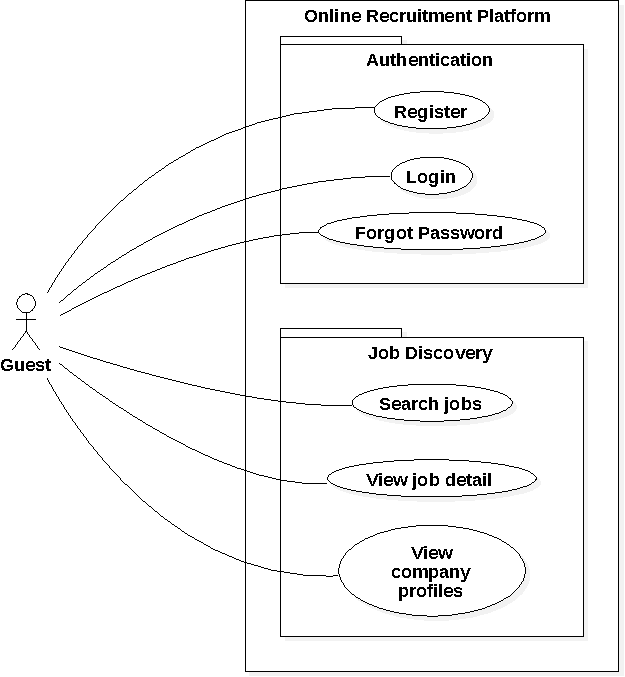
\includegraphics[width=0.5\linewidth]{diagrams/exported/Use Case/Guest Use Case-crop.pdf}
	\caption{Guest Use Case Diagram.}
	\label{diagram:uc-guest}
\end{figure}

\subsubsection{Authenticated User Use Cases}

Figure \ref{diagram:uc-authenticated} covers the functions common to all signed-in users: managing account information, changing the password, and logging out. Business-specific functions are introduced through the specialized actors in the next section.

\begin{figure}[H]
	\centering
	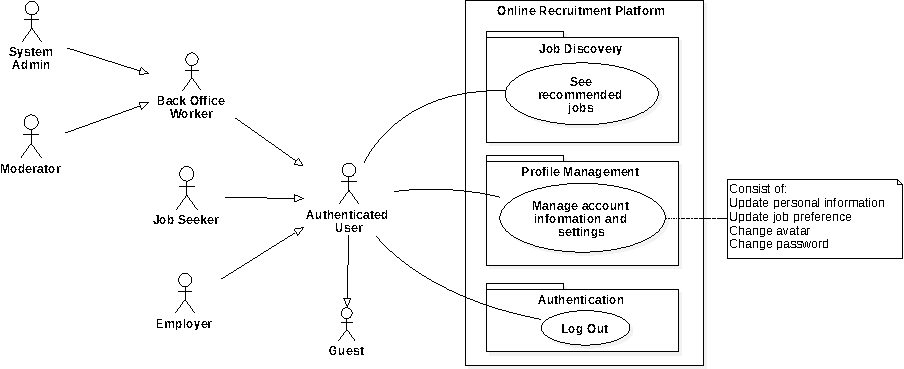
\includegraphics[width=\linewidth]{diagrams/exported/Use Case/Authenticated Use Case-crop.pdf}
	\caption{Authenticated User Use Case Diagram.}
	\label{diagram:uc-authenticated}
\end{figure}

\subsection{Specialized Use Cases}

The following subsections describe the use cases associated with each specialized actor. The Job Seeker and Employer actors correspond to the two modules examined in detail in this thesis, while the Back Office Worker supports the platform's administrative and moderation functions.

\subsubsection{Job Seeker Use Cases}

The Job Seeker is the main user on the demand side of the platform: this actor looks for jobs, manages their resume, and participates in recruitment through job applications.

\begin{figure}[H]
	\centering
	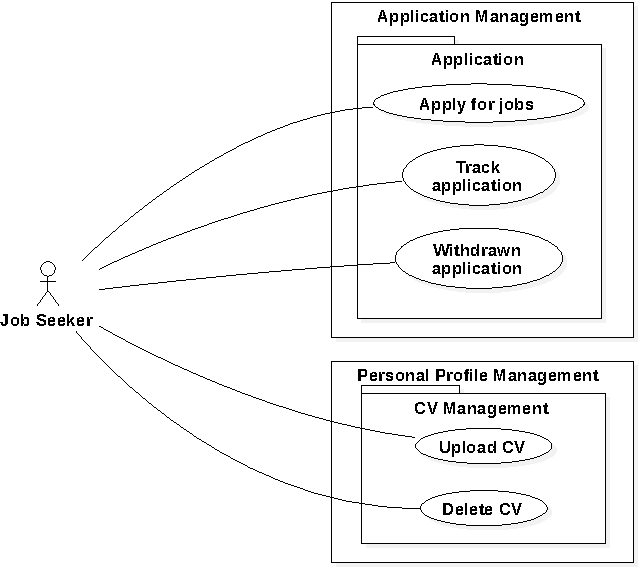
\includegraphics[width=0.7\linewidth]{diagrams/exported/Use Case/JS Use Case-crop.pdf}
	\caption{Job Seeker Use Case Diagram.}
	\label{diagram:uc-job_seeker}
\end{figure}

Figure \ref{diagram:uc-job_seeker} shows the Job Seeker's capabilities, including the CV Management and Application packages. The three application-related use cases: Applying, tracking, and withdrawing form the Job Application functionality examined in this thesis.

\subsubsection{Employer Use Cases}

The Employer represents the organizations and recruiters who publish job postings and evaluate applicants.

\begin{figure}[H]
	\centering
	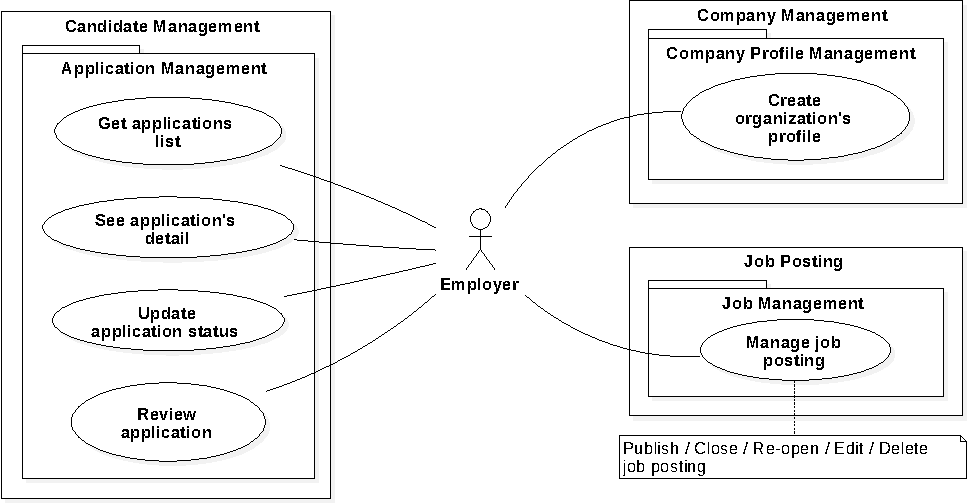
\includegraphics[width=\linewidth]{diagrams/exported/Use Case/Employer Use Case-crop.pdf}
	\caption{Employer Use Case Diagram.}
	\label{diagram:uc-employer}
\end{figure}

Figure \ref{diagram:uc-employer} shows the Employer's capabilities, including Company Profile Management, Job Management, and Application Management. These use cases collectively support the complete recruitment lifecycle on the employer's side, from creating a company profile and managing job postings to reviewing and updating the status of received applications. This functionality constitutes the Employer Job Management module examined in this thesis.

\subsubsection{Back Office Worker Use Cases}

The Back Office Worker, consist of Employer and System Administrator, represents internal personnel responsible for maintaining platform integrity and ensuring that the recruitment platform operates correctly.

\begin{figure}[H]
	\centering
	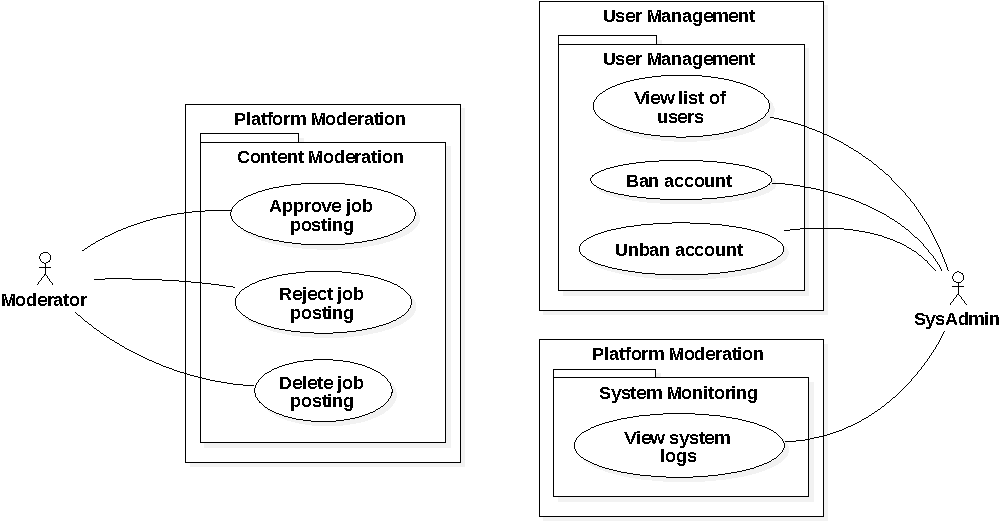
\includegraphics[width=\linewidth]{diagrams/exported/Use Case/Admin Use Case-crop.pdf}
	\caption{Back Office Worker Use Case Diagram.}
	\label{diagram:uc-back_office}
\end{figure}

Figure \ref{diagram:uc-back_office} show the Back Office Worker's capabilities, including Platform Moderation and User Management. These use cases highlight the supervisory tasks of the back office worker, from managing user's status, moderating job postings, and overseeing important system events through logs.

\section{Use Case Specification}

The use case diagrams above give an overview of the system's functional scope. This section specifies the main use cases of the two featured modules in detail.

\newpage
\subsection{Job Seeker: Apply for Job}

This subsection provides a detailed specification of the Apply for Job use case identified in the Job Application module.

\begin{usecasespectable}
	{Use Case Specification: Apply for Job.}
	{tab:ucs-apply_for_job}

	Use Case ID & UC-JS-01 \\ \hline

	Use Case Name & Apply for Job \\ \hline

	Primary Actor & Job Seeker \\ \hline

	Goal & Submit a job application to an employer. \\ \hline

	Description &
	Allows a Job Seeker to submit an application for a published job posting.
	\\ \hline

	Preconditions &
	\begin{itemize}
		\item Job Seeker is authenticated.
		\item The job posting is open for applications.
		\item Job Seeker has an uploaded resume.
	\end{itemize}
	\\ \hline

	Trigger &
	The Job Seeker selects the \textbf{Apply} option on a job posting.
	\\ \hline

	Main Success Scenario &
	\begin{enumerate}
		\item Job Seeker views the job posting.
		\item Job Seeker selects Apply.
		\item System displays the application form and the job summary.
		\item Job Seeker selects a resume.
		\item Job Seeker submits the application.
		\item System validates that the job is active, the resume belongs to the user, and no duplicate application exists.
		\item System records the application as \texttt{SUBMITTED}.
		\item System confirms the submission.
	\end{enumerate}
	\\ \hline

	Alternative Flows &
	\textbf{A1. No resume uploaded}
	\begin{enumerate}
		\item System asks the Job Seeker to upload a resume first.
	\end{enumerate}

	\textbf{A2. Already applied}
	\begin{enumerate}
		\item System rejects the submission.
		\item System informs the Job Seeker that an application already exists.
	\end{enumerate}

	\textbf{A3. Posting no longer active}
	\begin{enumerate}
		\item System rejects the submission.
		\item System informs the Job Seeker that the posting is no longer available.
	\end{enumerate}
	\\ \hline

	Postconditions &
	\begin{itemize}
		\item A new application with status \texttt{SUBMITTED} is created.
	\end{itemize}
	\\ \hline

\end{usecasespectable}

\newpage
\subsection{Employer: Publish Job Posting}

This subsection provides a detailed specification of the Publish Job Posting use case identified in the Employer Job Management module.

\begin{usecasespectable}
	{Use Case Specification: Publish Job Posting.}
	{tab:ucs-publish_job_posting}

	Use Case ID & UC-EMP-01 \\ \hline

	Use Case Name & Publish Job Posting \\ \hline

	Primary Actor & Employer \\ \hline

	Goal & Publish a job posting for potential applicants. \\ \hline

	Description &
	Allows an Employer to create and publish a new job posting.
	\\ \hline

	Preconditions &
	\begin{itemize}
		\item Employer is authenticated.
		\item Employer has a registered company profile.
	\end{itemize}
	\\ \hline

	Trigger &
	Employer selects the \textbf{Post a Job} function.
	\\ \hline

	Main Success Scenario &
	\begin{enumerate}
		\item Employer fills in the job title, description, requirements, location, employment type, and deadline.
		\item Employer submits the posting.
		\item System validates the input and checks that the deadline is in the future.
		\item System assigns the employer's company to the posting.
		\item System creates the posting with status \texttt{PENDING\_APPROVAL}.
		\item System confirms the creation and shows the posting in the employer's list.
	\end{enumerate}
	\\ \hline

	Alternative Flows &
	\textbf{A1. No company profile}
	\begin{enumerate}
		\item System requires the Employer to create a company profile first.
	\end{enumerate}

	\textbf{A2. Invalid input}
	\begin{enumerate}
		\item System identifies the invalid fields.
		\item Employer corrects and resubmits.
	\end{enumerate}
	\\ \hline

	Postconditions &
	\begin{itemize}
		\item A job posting with status \texttt{PENDING\_APPROVAL} is stored.
		\item The posting is hidden from public search until approved.
	\end{itemize}
	\\ \hline

\end{usecasespectable}

\newpage
\subsection{Employer: Review Application}

This subsection provides a detailed specification of the Review Application use case identified in the Employer Job Management module.

\begin{usecasespectable}
	{Use Case Specification: Review Application.}
	{tab:ucs-review_application}

	Use Case ID & UC-EMP-06, UC-EMP-07, UC-EMP-08 \\ \hline

	Use Case Name & Review Application \\ \hline

	Primary Actor & Employer \\ \hline

	Goal & Review the applications a posting received and update their status. \\ \hline

	Description &
	Allows an Employer to view the applications submitted to a posting and move each one through the review pipeline.
	\\ \hline

	Preconditions &
	\begin{itemize}
		\item Employer is authenticated.
		\item The posting belongs to the employer's company.
	\end{itemize}
	\\ \hline

	Trigger &
	Employer opens the application list of a job posting.
	\\ \hline

	Main Success Scenario &
	\begin{enumerate}
		\item Employer selects a job posting.
		\item System lists the applications with candidate name, resume, and status.
		\item Employer opens an application's detail.
		\item Employer marks the application \texttt{UNDER\_REVIEW}.
		\item Employer decides to accept or reject the application, with an optional reason on rejection.
		\item System updates the application to \texttt{ACCEPTED} or \texttt{REJECTED} and records the decision time.
	\end{enumerate}
	\\ \hline

	Alternative Flows &
	\textbf{A1. Application withdrawn}
	\begin{enumerate}
		\item System blocks further processing of the application.
	\end{enumerate}

	\textbf{A2. Application already decided}
	\begin{enumerate}
		\item System rejects the status change.
	\end{enumerate}

	\textbf{A3. Application not under review}
	\begin{enumerate}
		\item System only allows accept or reject on applications that are \texttt{UNDER\_REVIEW}.
	\end{enumerate}
	\\ \hline

	Postconditions &
	\begin{itemize}
		\item The application is \texttt{ACCEPTED} or \texttt{REJECTED}, with the decision time recorded.
	\end{itemize}
	\\ \hline

\end{usecasespectable}